\documentclass{article}
\usepackage{exercise}
\usepackage[obeyspaces]{url}
\usepackage[dvipsnames]{xcolor}
\usepackage{graphicx}
\usepackage{listings}
\usepackage[scaled]{helvet}
\usepackage{amsmath,amssymb,amsfonts,mathtools,cancel}

% typeset in helvetica
\renewcommand*\familydefault{\sfdefault}


% QE stuff
\def\qe{{\sc Quantum ESPRESSO}}
\def\pwx{\texttt{pw.x}}
\def\cpx{\texttt{cp.x}}
\def\phx{\texttt{ph.x}}
\def\nebx{\texttt{neb.x}}
\def\configure{\texttt{configure}}
\def\PWscf{\texttt{PWscf }}
\def\PHonon{\texttt{PHonon}}
\def\CP{\texttt{CP}}
\def\PostProc{\texttt{PostProc}}
\def\NEB{\texttt{PWneb}} % to be decided
\def\make{\texttt{make}}
%%%%%%%%%%%%%%%%%%%%%%%%

\def\ipi{i-PI}
\newcommand{\hints}[1]{\emph{Hints: #1}}
\newcommand{\lstinxml}{\lstinline[language=XML]}
\newcommand{\lstinbash}{\lstinline[language=Bash]}
\usepackage[space=true]{accsupp}

\newcommand{\pdfactualhex}[3]{\newcommand{#1}{%
\BeginAccSupp{method=hex,ActualText=#2}#3\EndAccSupp{}}}

% PASTABLE lstlisting code
\pdfactualhex{\pdfactualdspace}{2020}{\textperiodcentered\textperiodcentered}
\pdfactualhex{\pdfactualsquote}{27}{'}
\pdfactualhex{\pdfactualbtick}{60}{`}

\lstset{tabsize=4,basicstyle=\ttfamily,breaklines=true,columns=flexible,emptylines=10000}
\lstset{literate={'}{\pdfactualsquote}1
                 {`}{\pdfactualbtick}1
                 {\ \ }{\pdfactualdspace}2
}

\lstset{
    basicstyle=\ttfamily,
    keywordstyle=\color{BrickRed},
    commentstyle=\color{Gray},
    stringstyle=\color{black},
    emphstyle=\color{RedOrange},
    columns=flexible,
    showstringspaces=false,
    xleftmargin=1em,
    deletekeywords={bin,all}
}


\lstdefinelanguage{Bash}
{
   alsodigit={-,.},
   morekeywords={ cp2k.popt, lmp_ubuntu, i-pi, vmd, for, done, python, mpirun, touch, tail, trajworks, autocorr, awk, i-pi-mergebeadspdb, grep, head, cp, cd, cat, ls, pwd, bash, sed, mkdir, vi, sh}
   %morecomment=[s][\color{orange}]{#}{\}
}

%\lstdefinelanguage{Python}
%{
%    morecomment=[s][\color{orange}]{#}{\}
%}


\lstdefinelanguage{XML}
{
  morestring=[b][\color{RedOrange}]",
%  morestring=[s]{>}{<},
  morecomment=[s]{<?}{?>},
  morecomment=[s][\color{orange}]{<!--}{-->},
  identifierstyle=\color{BlueViolet},
  keywordstyle=\color{ForestGreen},
  stringstyle=\color{RedOrange},
%  tagstyle=\color{Blue},
  morekeywords={xmlns,version,type, mode, units, forcefield, filename, stride, overwrite, nbeads,prefix}% list your attributes here
}

\lstdefinestyle{XML}
{
\tagstyle=\color{Blue}
}

\title{An introduction to \ipi{}}
\author{Riccardo Petraglia, Michele Ceriotti}
\date{January 2017}

\setlength\parindent{0pt}

\begin{document}

\maketitle

% INTRO
In this set of exercises we will learn about the basics of \ipi\ and
its use jointly with \qe.

As may be already clear, \ipi\ is not meant to compute forces. Thus,
an external engine is needed. Once the external engine is set, \ipi\
takes care of the generation of the MD trajectory. This approach
is extremely flexible. For example different kind of forces can be
mixed within \ipi\ permitting the use of forces coming from different
sources: correcting terms from different software (\PWscf~+ external
dispersion correction) or multiple time step approaches with
expensive/cheap forces computations (see the Ring Polymer Contraction
method).

\begin{figure}[h!]
\centering
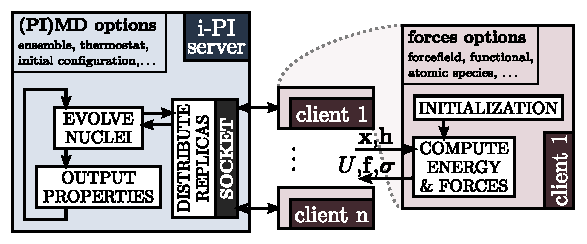
\includegraphics[width=0.9\textwidth]{ipi-scheme.pdf}
\caption{\ipi\ communicates with the force engine using sockets in a
  client/server fashion where \ipi\ behaves as the server. The engine
  connects to the server and provide \ipi\ the data it asks
  for.}\label{fig:ipi-scheme}
\end{figure}


The following exercises are created to increase the confidence of the user
with the \ipi\ workflow and to clarify the server/client approach on
which the \ipi-engine communication protocol is based (see
fig. \ref{fig:ipi-scheme}). Moreover, you will understand how to
set-up a simulation using the PIGLET thermostat to improve the Path
Integral Molecular Dynamics efficiency.

\begin{Exercise}[label={i-pi},title={Molecular Dynamics: a client/server approach}]

In this exercise, we will perform a simple Molecular Dynamics (MD)
calculation using \PWscf\ as engine. Since the computation of QM forces is
expensive, here we use a single molecule of water in gas phase. Moreover, the
\PWscf\ input is prepared sacrificing its accuracy to run faster.

The simulation will be performed using the NVT ensemble at 300K.  We
will also record the kinetic and potential energy and the conserved
quantity of the system and the positions of the atoms.

\Question
Read the \PWscf\ input file \url{ex-1/pw.in}.
Is there any difference in respect of a plain single point computation?
How is told to \pwx\ where to find the \ipi\ server?\\

The input of \pwx\ is a valid input to run a single point
computation. To make \pwx\ aware of \ipi, you should specify an option
when calling the software (see section 3.6 of PWscf user's manual).
\begin{lstlisting}[language=bash]
pw.x --ipi host:port < pw.in
\end{lstlisting}
The forces are then computed by \pwx\ at the level of electron theory
specified in the input and passed to \ipi\ thought the socket
interface.

\Question
Open the \ipi\ input file \url{ex-1/ipi.xml}. Specifying in
the input which is the address of the socket where \ipi\ will wait for a \pwx\
instance is essential. You have two possibilities: using a UNIX-domain
or an INET-domain socket. The former is faster but the server and the
client must run on the same machine. The latter allows communication
through the ``internet'' so that \ipi\ and the ``force
calculator'' can run on a different computer.

The following steps tell \ipi\ to wait for a client connecting on the UNIX
socket called \texttt{single-water-qe}. Look for the following snippet
in the \url{ex-1/ipi.xml}:
\begin{lstlisting}[language=xml]
<ffsocket name="..." mode="unix">
<address>...</address>
</ffsocket>
\end{lstlisting}
Edit the file replacing the dots with appropriate values. Any string
would be fine but, if you
want to be consistent with the rest of the tutorial, you should use
the following:
\begin{table}[h!]
  \centering
  \begin{tabular}{ccc}
    \texttt{name} & $\longrightarrow$ & \texttt{pw-forces}\\
    \texttt{address} & $\longrightarrow$ & \texttt{single-water-qe}
  \end{tabular}
\end{table}


\textbf{Pay attention that attribute's values must be within single- or
double-quotes!}\\


The \texttt{name} attribute in the \texttt{ffsocket} node assigns a
reference to the forcefield within the \ipi\ input. This reference
will be used to specify the origin of the force within the
\texttt{system} node.

\Question
Introduce a \texttt{<force>} node that references to the previously 
 defined \texttt{<ffsocket>}.

\ipi\ can manage different simulations at the same time. Each
simulation is defined in the \texttt{<system>} node. Each
\texttt{<system>} can also use forces coming from different 
calculators. Since this is an introductory course, we are going to use
a single system with a single force. In the file \url{ex-1/ipi.xml}
look for the following snippet:
\begin{lstlisting}[language=xml]
<forces>
<force forcefield='...'/>
</forces>
\end{lstlisting}
Replace the three dots with the name of the forcefield you want to use
to compute the forces in this system. If you used the names suggested
in the tutorial, it should be \texttt{pw-forces}.

\Question
We are now ready to run the simulation.\\

The first thing to do is to start the \ipi\ server. Use the following
command when in the folder \url{ex-1}:
\begin{lstlisting}[language=bash]
i-pi ipi.xml
\end{lstlisting}
If everything is fine, the shell will show some messages and will stop
with the following string:
\begin{lstlisting}[language=bash]
Created unix socket with address single-water-qe
@ForceField: Starting the polling thread main loop
\end{lstlisting}
this means that the server started correctly and is waiting for a
client that computes forces.

To start \pwx\ as an \ipi\ client open a new terminal, enter the
folder \url{ex-1} and create a new directory. Enter the just
created folder and run the
following command after replacing the \texttt{unix\_address} with the
actual address where \ipi\ is waiting (if followed tutorial
suggestions, this should be \texttt{pw-forces}):
\begin{lstlisting}[language=bash]
pw.x --ipi unix_address:UNIX < pw.in
\end{lstlisting}


\Question
Now switch to the terminal where \ipi\ is running, notice
that \ipi\ has built the connection with \pwx:
\begin{lstlisting}[language=sh]
 @SOCKET:   Client asked for connection from . Now hand-shaking.
 @SOCKET:   Handshaking was successful. Added to the client list.
\end{lstlisting}
and started the Molecular Dynamics simulation.
It should also dump out information on the time cost of each MD step.

\Question
Try to kill the \pwx\ instance.  Simply switch to the
terminal where \pwx\ is running and press \url{Ctrl+c}.  Now look at
whether \ipi\ is still running.  Notice that although the evolution of
MD is paused, \ipi\ itself does not die off but instead continue to
run and wait for new client to take over.  Now start \pwx\ again using
the previous command.
What happens to \ipi\ now?  \ldots Nice eh?


\Question
What if one stops \ipi ?  Kill \ipi\ by typing \url{Ctrl+c}
where it is running, or create a file named \url{EXIT} in the folder
where \ipi\ is running (you can use the bash command \texttt{touch
  EXIT}).  Watch how \ipi\ responds, and how \pwx\ reacts.  Think
about what are the advantages of a clean exit when a MD program stops
unexpectedly.


\Question
Checking the \texttt{<initialization>} node in the \ipi\ input, we see
the attribute \texttt{nbeads=4}. This means that we are running a Path
Integral Molecular Dynamics (PIMD) simulation with 4 beads. Easy, isn't it?.
This explains why \ipi\ is producing so many xyz files as output. There
is an output for each bead and a fifth file containing the trajectory
of the centroid. You can open them all together with the following
command:
\begin{lstlisting}[language=bash]
vmd -m example*.xyz
\end{lstlisting}
You can also look at the \url{ex-1/example.out} file. This is the
result of the \texttt{<property>} node. The header of the file
summarizes what is printed in each column. You can create a graph using
the following command:
\begin{lstlisting}[language=bash]
plot example.out -1,3
\end{lstlisting}
The \texttt{-1,3} keyword tells to the script to use the column 1 as
x-axis and the column 3 as y-axis. You can discover more option simply
writing \texttt{plot} and pressing enter.
\end{Exercise}
\vspace{1em}

Before starting with the next exercise, take a few minutes to explore
all the other keyword in the \ipi\ input. If you are familiar with
other MD software, you should find the input quite self-explaining.
Try to focus also on the \texttt{<output>} node and understand why
\ipi\ is printing all those files.


When you are tired of looking at a single molecule of water, go to the
next exercise.

MD simulations are quite computationally expensive and performing
simulation with \emph{ab-initio} force evaluation would require much
more time than what you can afford during this tutorial. This is why,
from now on, the code LAMMPS will be used instead of \qe. All the
input for \qe\ will anyway be present in the exercise \texttt{run} folders.

\vspace{2em}

\begin{Exercise}[label={inputs},title={Liquid water with the
    \emph{PIGLET} thermostat}]
In this exercise you are going to learn how to perform a PIMD
simulation using the PIGLET thermostat to improve the efficiency of
the sampling.

\Question
Open the \ipi\ input file at \url{ex-2/ipi.xml} and localize the node
describing the thermostat. The attribute \texttt{mode} of the
thermostat is set to \texttt{langevin}. The PIGLET thermostat requires
some parameters that can be downloaded from the following website
\url{https://epfl-cosmo.github.io/gle4md/index.html?page=matrix}.
To obtain the right parameters do the following:
\begin{enumerate}
\item Select \texttt{PIGLET} as \textbf{GLE type};
\item Set the number of beads \textbf{N. beads} to \texttt{6};
\item The \textbf{Par. set} should be \texttt{Ns=8,
    $\hbar\omega/kT=20$, PIGLET}
\item To get the output in the \ipi\ input form, select \ipi\ in the
  \textbf{Output format}.
\item All the other parameters are left to the default value.
\end{enumerate}
In this context, the \texttt{Ns} are the number of degrees of freedom
of the bath, $\omega_{max}$ and \texttt{centroid} are the maximum
and the window frequencies for which the sampling is
enhanced. \textbf{Target T} is the temperature of the simulation and
$\hbar\omega/KT$ is the ratio between vibrational energy and average
kinetic energy.

Before proceeding further, do a copy of the entire directory
\url{ex-2} and call it \url{ex-2-piglet}. Enter this latter and
replace the langevin thermostat (all the \texttt{thermostat} node must
be substituted) into the file \url{ex-2-piglet/ipi.xml} with the code
obtained from the website.

\Question
Change the \texttt{verbosity} value from \texttt{medium} to
\texttt{high} and start \ipi\ with the following command:
\begin{lstlisting}[language=bash]
i-pi ipi.xml
\end{lstlisting}
from the \url{ex-2-piglet} folder.

At this point you have two choices for the force provider: you start
\PWscf\ or LAMMPS. Since this simulation contains 96 atoms, we warmly
suggest using LAMMPS in this test by running the following command:
\begin{lstlisting}[language=bash]
lmp_serial -i in.water
\end{lstlisting}
in a different shell. While the simulation is running, in order to
understand the \ipi\ machinery better, you could prepare a \pwx\ input
for this example starting from the \pwx\ input provided in the folder
\url{ex-1/pw.in}. Try also to run it with \ipi\ to be sure it's working.

What are the lines inside the LAMMPS input which set the communication
with \ipi ?

\Question
Stop LAMMS (press \url{Ctrl+c} in the terminal where it has been
ran). \ipi\ is now waiting for a new connection. Restart LAMMPS with
the following command:
\begin{lstlisting}[language=bash]
lmp_serial -i in.water > lmp.out.1 &
\end{lstlisting}
The shell should still present you the prompt. Run the same command a
second time replacing the last ``1'' with a ``2''. What is happening
in the \ipi\ terminal? You can see that now \ipi\ prints out much more
information. Can you understand what they are? How many instances of
LAMMPS could be used to maximize the performances?

\end{Exercise}

With this second exercise we performed a much more interesting
simulation using some advanced method to increase the efficiency of
the PIMD statistical sampling. Before moving to the next exercise, we
strongly suggest to run the same simulation using a white noise Langevin
thermostat and a single bead (classical dynamics).  Let both run while
working on the next exercise. We will come back to these at the end of
the tutorial to analyze some results.

At this point, you should know \ipi\ well enough to
proceed with the next simulation without much help. Pay attention to
the fact that only one instance of \ipi\ can use a given socket at
time. If you want to run two \ipi\ server at the same time, make sure
they have a different \texttt{<address>} or, in the case of INET domain
sockets, at least different \texttt{<port>}. At the end, you can look
at the differences between the two trajectories.

\vspace{2em}

\begin{Exercise}[label={inputs},title={PIMD-NPT simulation of ice}]
The goal of this exercise is to run a PIMD simulation in the NPT
ensemble. The \ipi\ input provided with the file \url{ex-3/ipi.xml} is
a valid input for a PIMD-NVT simulation. The idea is to transform it
in a valid input for a PIMD-NPT simulation.

\Question
Take a look at the input provided and identify the nodes responsible
for the task \ipi\ will perform.
\texttt{motion} is the most important node in this case.
Look at the following snippet:
\begin{lstlisting}[language=xml]
<motion mode='dynamics'>
<dynamics mode='nvt'>
<thermostat mode='langevin'>
<tau units='femtosecond'> 100 </tau>
</thermostat>
<timestep units='femtosecond'> 0.25 </timestep>
</dynamics>
</motion>
\end{lstlisting}
This section of the input tells \ipi\ that the computation we want to
perform is a molecular \texttt{dynamics}, in the \texttt{nvt} ensemble
using a \texttt{langevin thermostat} and a \texttt{timestep} of 0.25
femtosecond.

There is also another important section:
\begin{lstlisting}[language=xml]
<ensemble>
<temperature units='kelvin'> 200 </temperature>
</ensemble>
\end{lstlisting}
This node of the input define all the ensemble properties. In the
case you want to perform an NPT simulation, the pressure must be
defined within the \texttt{ensemble} node.


\Question
Add a barostat. You can follow the user guide to understand how to
set-up the barostat. Anyway, the following snippet provide a general setup
which is suitable for this case.
\begin{lstlisting}[language=xml]
<barostat mode='isotropic'>
<tau units='femtosecond'> 200</tau>
<thermostat mode='langevin'>
<tau units='femtosecond'> 100</tau>
</thermostat>
<h0> [ 25.6156, 0, 0, 0, 29.5783, 0, 0, 0, 27.8867 ]</h0>
</barostat>
\end{lstlisting}
Where is the place for this node? The \texttt{barostat} is a
characteristic of the \texttt{dynamics} itself. Then it must be
specified within that node. Copy the snippet aforementioned and paste
just before the \texttt{<timestep>} node.


\Question What if we want to perform an NPT simulation with an
anisotropic barostat? This kind of simulations need an extension of
the NPT ensemble, called NST (constant-temperature,
constant-stress). Thus, in \ipi\ set the attribute \texttt{mode} of
the \texttt{dynamic} node to \texttt{nst}. This means also that the
\texttt{<ensemble>} node must contain a stress tensor instead of an
isotropic pressure. To simulate our system with an anisotropic cell at
atmospheric pressure, use the following snippet inside the
\texttt{<ensamble>} node:
\begin{lstlisting}[language=xml]
<stress units='megapascal'> [10, 0, 0, 0, 10, 0, 0, 0, 10] </stress>
\end{lstlisting}
The stress is a 3x3 tensor. To simplify user's life, this kind of tensors are 
flatten in the \ipi input.

At this point the input is ready to perform a simulation with at
``constant anisotropic pressure''.

\Question
What does the list \texttt{h0} contains? Why do we need a thermostat
within the barostat?

The list of numbers is a reference cell for the Parrinello-Rahman
barostat (which is the one implemented in \ipi). In practice, those
numbers are the dimension of the cell that must be written into the xyz
input file (\url{ex3-1/init.xyz}) or in the pdb file (take as an
example the one at \url{ex1/h2o-init.pdb}). The coordinate files
also contains the units of dimension of the cell and the positions
(\texttt{cell\{angstrom\}} and \texttt{position\{angstrom\}}).

\Question
Following the same procedure used in the last exercise, start this
simulation.

\end{Exercise}

\begin{Exercise}[label={inputs},title={Radial distribution function comparison}]
As a last exercise, you should compare the radial distribution
function obtained from the two simulation of exercise 2.

\Question
Compute radial distribution functions for the different simulations. You
can use any tool of your liking, but we suggest the \url{trajworks}
post-processing tool that is part of the \url{toolbox} library.
Run the following command in the two folders used during the exercise
2: \url{ex-2} and \url{ex-2-piglet}.
\begin{lstlisting}[language=bash]
$read_box <(tail -q -n +100 example.pos_*.xyz) > box.dat%$
$tail -q -n +100 example.pos_*.xyz | trajworks -ixyz \
        -box box.dat -gr -gr1 O -gr2 O -grmax 5 -grbins 250 -hwin \
        triangle  -hwinfac 2 > gOO.dat%$
\end{lstlisting}

To visualize the result you can use the \texttt{plot} command from
\url{ex-2-piglet} folder:
\begin{lstlisting}[language=bash]
plot gOO.dat ../ex-2-langevin/gOO.dat -1,2
\end{lstlisting}
Also compute the O--H radial distribution function.
Do you see any difference? Can you explain why?

\end{Exercise}

We hope this tutorial made you familiar with the use of \ipi. You
can find more tutorials and more information (as well as a link to the
last development and stable versions at \url{http://ipi-code.org}.

% \noindent In this exercise we are going to familiarize ourselves with the important notations of \ipi\ input files.
% Let"s take a look at the input files in the folder \url{ex-2}.
% The simulation system of choice here is one gas phase water molecule using NVT ensemble at 300K.


% \Question
% Let"s take a close look at the units first - which are the source of many errors during simulation and analysis.
% All the units used internally by \ipi\ are atomic units, as given
% below.

% \texttt{
% \begin{center}
% \begin{tabular}{lll}
% \hline\hline
% Unit & Name & S.I. Value\\
% \hline
% Length & Bohr radius & 5.2917721e-11 m\\
% Time & N.A. & 2.4188843e-17 s\\
% Mass & Electron mass & 9.1093819e-31 kg\\
% Temperature & Hartree & 315774.66 K\\
% Energy & Hartree & 4.3597438e-18 J\\
% Pressure & N.A. & 2.9421912e13 Pa\\
% \hline\hline
% \end{tabular}
% %\par\end{center}
% \end{center}
% }

% By default, both input and output data are given in atomic
% units, but in most cases the default units can be overridden if one
% wishes so.
% For example, in \url{ex-2/input.xml}
% we used
% \begin{lstlisting}[language=xml]
% <properties stride="1" filename="out">
% [ step, time{picosecond}, conserved, temperature{kelvin}, potential ]
% </properties>
% <trajectory filename="xc" stride="1"> x_centroid{angstrom}
% </trajectory>
% \end{lstlisting}
% so that the time, temperature, and the trajectory will written out in the units of picosecond, Kelvin, and Angstrom in the output files, respectively.
% Similarly, the units of the initialization files can be specified such as
% \begin{lstlisting}[language=xml]
% <file mode="xyz" units="angstrom"> h2o.xyz </file>
% <cell mode="abc" units="angstrom"> [ 8, 8, 8 ] </cell>
% <velocities mode="thermal" units="kelvin"> 300 </velocities>
% \end{lstlisting}
% When using \ipi\, you can play around with the units to facilitate the initialization process as well as subsequent analyses.

% \Question
% Now we will observe the format and structure of \url{input.xml}.
% The xml file consists of a set of hierarchically nested tags. There are three
% parts to an xml tag. Each tag is identified by a tag name, which specifies the class
% or variable that is being initialized. Between the opening and closing tags there is some data,
% which is used to specify the
% contents of a class object, or the value of a variable. Finally tags can have attributes,
% which are used to specify how the tag should be interpreted.
% A xml tag has the following syntax:
% \begin{lstlisting}[language=xml]
% <tag_name attrib_name=attrib_data>tag_data</tag_name>
% \end{lstlisting}
% For example, in the tag
% \begin{lstlisting}[language=xml]
% <thermostat mode="pile_l">
% <tau units="femtosecond">100</tau>
% <pile_lambda>0.1</pile_lambda>
% </thermostat>
% \end{lstlisting}
% the tag name \lstinxml{thermostat} indicates which part of the simulation options is being defined,
% \lstinxml{mode="pile_l"} specifies the type of thermostat in use,
% and \lstinxml{<tau units="femtosecond">100</tau>} is used to set the parameters used for this particular thermostat.
% Please browse around this \url{input.xml} to see if you can make sense of most of the attributes.

% \Question
% It is worth spending a bit more time to explain about the type of socket used here.
% For the communication between \ipi\ and client codes, both Internet and Unix domain sockets can be used: the
% latter allow for fast communication on a single node, whereas the former make it possible
% to run \ipi\ and the clients on different computers.
% Here we demostate how to use the Internet (TCP/IP) sockets.
% In \ipi\ inout file we have
% \begin{lstlisting}[language=xml]
% <ffsocket mode="inet" name="cp2k">
% <latency> 1.00e-02</latency>
% <slots> 4 </slots>
% <port> 20614 </port>
% <timeout>  6.00000000e+02 </timeout>
% <address> localhost </address>
% </ffsocket>
% \end{lstlisting}
% and in CP2K input file \url{cp2k.in} we have the following
% \begin{lstlisting}[language=bash]
% &MOTION
% &DRIVER
% HOST localhost
% PORT 20614
% &END DRIVER
% &END MOTION
% \end{lstlisting}
% The above means that an Internet domain socket with port number 20614 is used for the communication.
% The port number is an integer between 1 and 32767 used to distinguish between all the
% different sockets open on a particular host. As many of the lower numbers are reserved
% for use in important system processes or Internet communication, it is generally advisable
% to only use numbers in the range 1025-32767 for simulations.

% \Question
% Now let"s see whether the Internet domain socket can indeed connect.
% Type the following to start \ipi\ and CP2K:
% \begin{lstlisting}[language=bash]
% $ i-pi input.xml &> log.ipi &
% $ cp2k.popt -o h2o.out cp2k.in &
% \end{lstlisting}
% Does it work? If you have access to two computers that can communicate with each
% other on the same network, you can try to run in a distributed-computing mode,
% with i-PI running on one computer and CP2K on the other. This advanced mode of
% operation, however, can be complex in the presence of firewalls or multiple
% network interfaces (see the i-PI documentation for some examples).

% \end{Exercise}

% \begin{Exercise}[label={water},title={Benchmark of quantum effects in a water molecule}]
% \noindent In this exercise we will perform a series of PIMD calculations to observe and benchmark nuclear quantum effects in a molecular system. Our system of choice will be a single molecule of water in vacuum so that simulations don"t take too much time and memory. We will be sampling an NVT ensemble using a q-TIP4P forcefield implemented within Lammps. We will look at the change in the kinetic and potential energy and the Oxygen--Hydrogen pair distribution function as we simulate in the quantum regime.

% \Question
% Look at the \ipi\ input file in \url{n.01/input.xml}. It is an \ipi\ input for a molecular dynamics simulations. Observe the
% properties and trajectory files that are specified in the \lstinxml$<output></output>$ section. From the previous exercise,
% it should be clear that the quantum kinetic and potential energy will be printed out every $4$ MD steps as columns $4$ and $5$ in the \lstinbash{$prefix.out} file. To compute the Oxygen--Hydrogen pair distribution function we shall also print out the positions of the atoms every $40$ MD steps int the \lstinbash{$prefix.pos_0} file.

% \Question
% Observe the \lstinxml$<initialize></initialize>$ section. We will be initialzing from a checkpoint file
% \lstinbash{start.chk} which is basically a RESTART file of a long equilibration run.
% From the previous exercise, it should be clear that the option \lstinbash{nbeads} should be $1$ for a classical simulation.

% \begin{lstlisting}[language=xml]
% <initialize nbeads="1">
% <file mode="chk"> init.chk </file>
% </initialize>
% \end{lstlisting}

% \Question
% Observe the \lstinxml$<motion></motion>$ section. The tags within the section should be
% verbose enough to help you interpret their meaning. We will be using a PILE-L thermostat~\cite{ceri+10jcp}
%  which for the case of a classical simulation reduces to a white noise Langevin thermostat.
% To be consistent with the rest of the PIMD runs, we will use an over-conservative time step of $0.25$fs.

% \Question
% To run the simulation launch \ipi\ and lammps in background. It is advisable to keep separate
% logs as useful information can be extracted from them.
% \begin{lstlisting}[language=bash]
% $ i-pi input.xml &> log.ipi &
% $ lmp_ubuntu < in.lmp &> log.lmp &
% \end{lstlisting}
% To compute the average values of the observable use the program called \url{autocorr} which takes a time series as an input and evaluates its auto-correlation function. It requires a mandatory flag called \url{-maxlag} which is the cutoff at the auto-correlation function is truncated. In addition to that it also computes the average and the associated error. Assuming that \lstinbash{$prefix} is the prefix used in \ipi\ input \begin{lstlisting}[language=bash]
% $ awk '!/#/{ print $6}' $prefix.out | tail -n +100 | \
%  autocorr -maxlag 10 | head
% \end{lstlisting}

% \Question
% To compute the Oxygen--Hydrogen pair correlation function we suggest you to use \url{trajworks} and follow the syntax as shown.
% \begin{lstlisting}[language=bash]
% $ cat $prefix.pos_0.xyz | trajworks -ixyz -box boxfile \
%  -gr -gr1 O -gr2 H -grmax 2 -grbins 200 -hwin triangle \
%  -hwinfac 2 > gOH.data
% \end{lstlisting}
% The \url{-gr} flag activates the computation of a pair correlation for atom types given by \url{-gr1} and \url{-gr2} until a maximum distance given by \url{-grmax} with a resolution given by \url{-grbins} grid points. The flags \url{-hwin} and \url{-hwinfac} indicate smoothening options.

% \Question
% Now go one folder up, and create new folder, copying all the input files
% for \lstinbash{n.01}. You can obtain an equilibrated
% of the extended system of 32 replicas of our system from
% \lstinbash{n.32/init.chk}.

% \begin{lstlisting}[language=bash]
% $ mkdir pi-test
% $ cp n.01/input.xml n.01/*.lmp pi-test
% $ cp n.32/init.chk pi-test
% $ cd pi-test
% \end{lstlisting}

% \Question
% Modify the input files so that you will run a PIMD calculation with 32 beads.
% Make the modifications as indicated by the comments in the xml snippet.
% \begin{lstlisting}[language=xml]
% <!-- change nbeads to 32-->
% <initialize nbeads="1">
% <file mode="chk" units="angstrom"> init.chk </file>
% </initialize>

% <ffsocket mode="unix" pbc="false" name="driver">
% <!-- change the addess to driver.32-->
% <address>driver.01</address>
% <port>31400</port>
% <latency>0.001</latency> <timeout>400</timeout>
% </ffsocket>
% \end{lstlisting}

% \Question
% Do not forget to change the address in the lammps input file.
% The comments in the following snippet should guide you.
% \begin{lstlisting}[language=sh]
% neighbor 2.0 bin
% timestep 0.00025
% # replace driver.01 with driver.32
% fix 1 all ipi driver.01 32346 unix
% run 100000000
% \end{lstlisting}

% \Question
% The folders \lstinbash{n.*} have already been prepared for you to run simulations with
% increasing numbers of beads. You should start one PIMD calculation in each of those folders.
% Compute the pair correlation function and the energy for all the simulations using \url{autocorr} and \url{trajworks}.


% \Question
% If you are late and want to save some time you could use the scripts provided --
% called \url{extract-pot.bash}, \url{extract-kin.bash} and \url{extract-gOH.bash}
% that are present in parent directory. These compute the potential energy,
% kinetic energy and the pair correlation function respectively.
% \begin{lstlisting}[language=bash]
% $ ls *.bash
% extract-gOH.bash extract-kin.bash extract-pot.bash
% \end{lstlisting}


% \Question
% Executing \url{extract-pot.bash} and \url{extract-kin.bash} will generate the average value and the error associated with the respective observable tabulated against the number of beads. What are the units? \hints{Have a look at the header of the output files
% of \ipi\. Unless otherwise specified, all outputs are in atomic units.}
% \begin{lstlisting}[language=bash]
% $ pwd
% tutorial-pimd16/day-1/ex-3
% $ bash extract-pot.bash > pot.data
% $ cat pot.data
% #nbeads avg error
%  1 4.822881e-02 5.040868e-03
%  2 7.203741e-02 4.090793e-03
%  4 1.453003e-01 4.452056e-03
%  8 2.191862e-01 4.346367e-03
% 16 2.533971e-01 2.726154e-03
% 32 2.812411e-01 1.435196e-02
% 64 3.046206e-01 7.312336e-03
% \end{lstlisting}
% To plot the average estimates with errors bars launch \url{gnuplot} and type the following
% \begin{lstlisting}[language=bash]
% > p "pot.data" us 1:2:3 w errorl
% \end{lstlisting}
% You should observe that the kinetic and potential energy individually converge to their quantum limit for \url{nbeads} $\sim 32$.

% \Question
% Executing \url{extract-gOH.bash} and \url{extract-kin.bash} will a file called gOH.data inside each of the sub directories \lstinbash{n.*}.
% \begin{lstlisting}[language=bash]
% $ pwd
% tutorial-pimd16/day-1/ex-3
% $ bash extract-gOH.bash
% $ ls */gOH.data
% n.01/gOH.data n.02/gOH.data n.04/gOH.data \
% n.08/gOH.data n.16/gOH.data n.32/gOH.data n.64/gOH.data
% \end{lstlisting}
% We suggest you to plot each of the pair distribution functions and see how they converge with number of beads. Launch \url{gnuplot} and type the following to

% \begin{lstlisting}[language=bash]
% > p "n.01/gOH.data" u 1:2 w l, "n.02/gOH.data" u 1:2 w l,\
%  "n.04/gOH.data" u 1:2 w l, "n.08/gOH.data" u 1:2 w l,\
%  "n.16/gOH.data" u 1:2 w l, "n.32/gOH.data" u 1:2 w l,\
%  "n.64/gOH.data" u 1:2 w l
% \end{lstlisting}
% You should observe the broadening of the probability distributions as you approach the quantum limit.
% \end{Exercise}

% \begin{Exercise}[label={ch5},title={PIMD in the strong quantum regime:  gas phase Methanium}]
% \noindent Having benchmarked nuclear quantum effects in a water molecule at room temperature
% we will study a $\text{CH}_{5}^{+}$ at 100 K where quantum effects such as tunneling and
% zero point fluctuations become strong. For a water molecule at $300$K, $\approx$32 beads were
% sufficient to accommodate NQEs, however in this case we will use $128$ beads since at low
% temperature quantum effects are stronger \hints{(Remember: the error in primitive PIMD
% converges as $(T/P)^2$)}. In other words, this simulation is $128$ times more computationally
% demanding than classical MD. We shall be sampling a \emph{NVT} ensemble and will monitor the
% proton delocalization by computing the Hydrogen--Hydrogen pair distribution function. For the
% purpose of comparison we will also run a cheap MD.

% \Question
% Move to the directory \url{ex-4/} and carefully observe the \ipi\ input files \url{n.001/input.xml}
% and \url{n.128/input.xml}. You will be initializing from an already thermalized restart file called
% \url{init.chk}. We shall also be printing out the trajectory every $1$fs so that we have enough
% statistics to compute the Hydrogen--Hydrogen pair distribution function. Run the classical and
% quantum simulations in their respective directories.

% \begin{lstlisting}[language=bash]
% $ i-pi input.xml &> log.ipi &
% $ cp2k.popt in.cp2k &> log.cp2k &
% \end{lstlisting}

% \Question
% To compute the Hydrogen--Hydrogen pair correlation function we suggest you to use \url{trajworks} and follow the syntax as shown.
% \begin{lstlisting}[language=bash]
% $ cat $prefix.pos_* | trajworks -ipdb -vbox -gr -gr1 H\
%  -gr2 H -grmax 3 -hwin triangle -hwinfac 5  > gHH.data
% \end{lstlisting}

% \Question
% You can use \url{gnuplot} to observe the difference int the pair distributions functions with and without PIMD.
% Launch gnuplot by typing \url{gnuplot} on the terminal and execute the following statement
% \begin{lstlisting}[language=bash]
% > p "n.128/gHH.data" u 1:2 w l, "n.001/gHH.data" u 1:2 w l
% \end{lstlisting}

% \end{Exercise}

%\bibliographystyle{unsrt}
%\bibliography{biblio}
\end{document}
